\begin{frame}
    \frametitle{Modelo de datos}

    \begin{block}{Estructura de datos}
        Un documento es una estructura que representa un objeto de la realidad. Un documento se considera una colección
        de pares llave-valor, los formatos más conocidos para su almacenamiento son JSON, BSON y XML.

        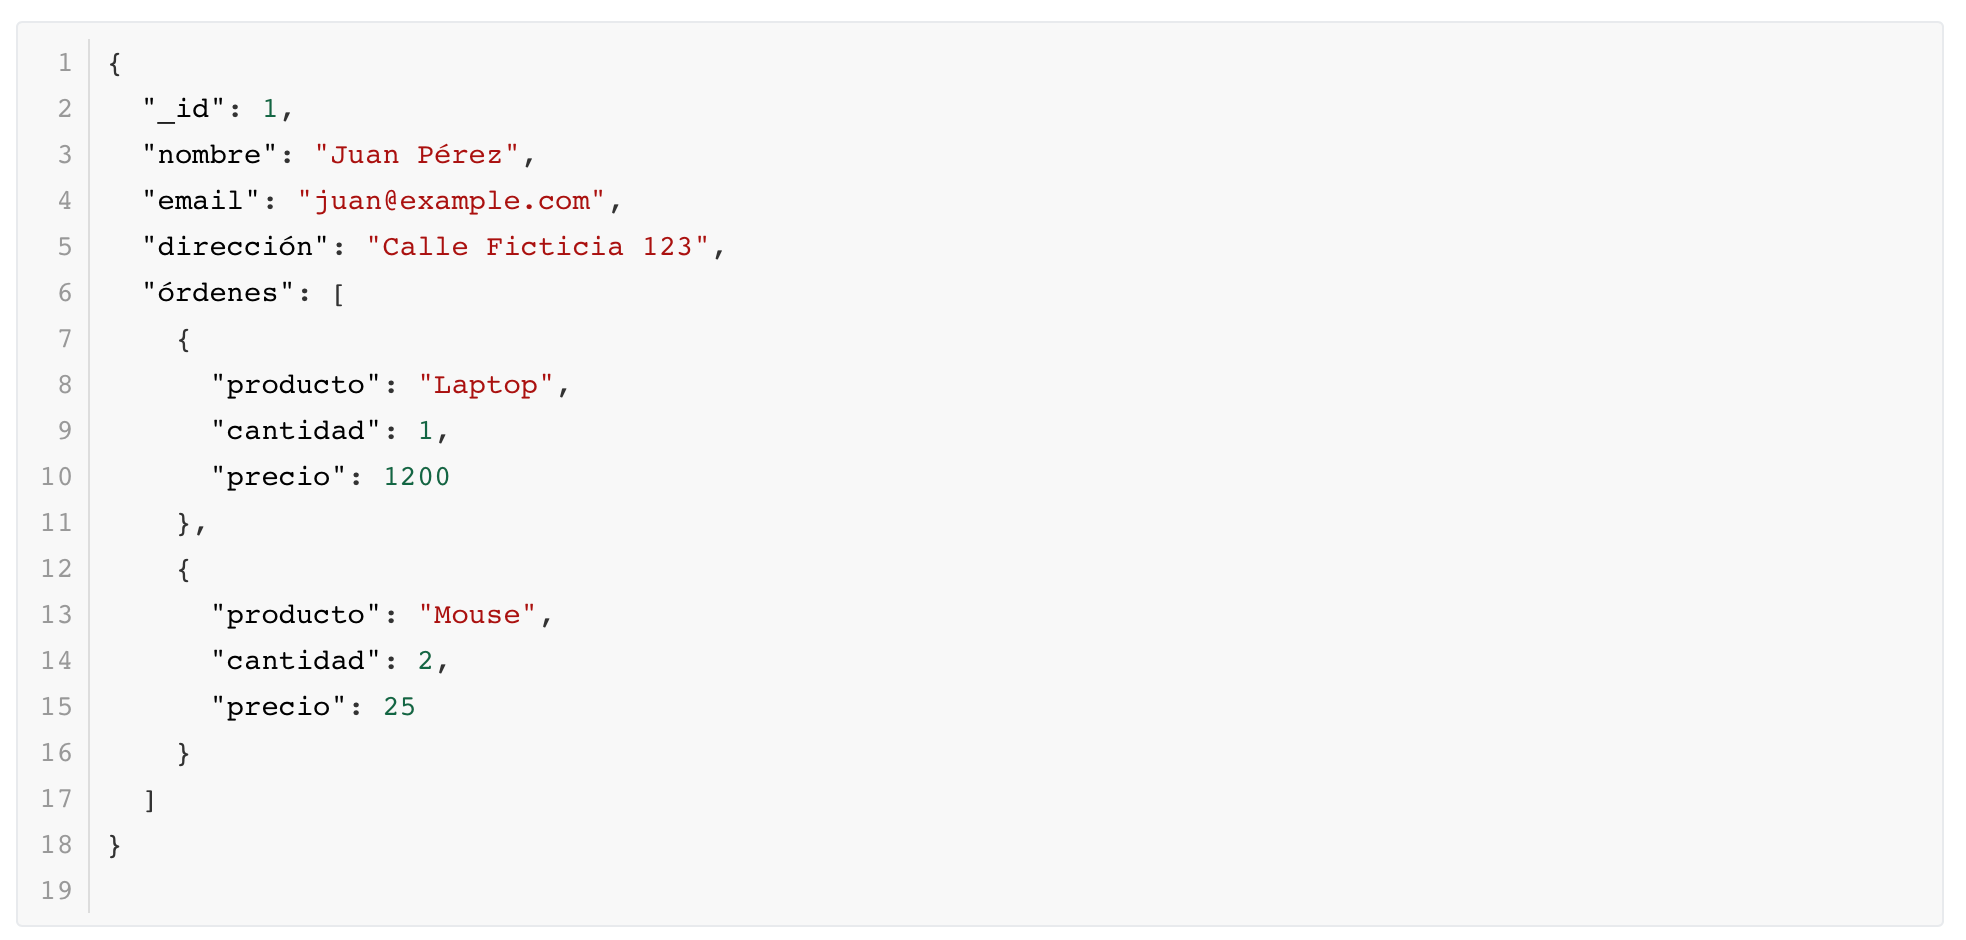
\includegraphics[width=0.8\textwidth]{img/json-example.png}
    \end{block}

    \note<1>{@NOTE x ejemplo:
        \begin{itemize}
            \item referenciar a valores \'unicos
            \item eliminar redundancia en datos repetidos continuamente (Run-Length Encoding)
            \item eliminaci\'on de nulls llevando m\'ascaras de bits, por ejemplo
        \end{itemize}
    }
\end{frame}

\begin{frame}
    \frametitle{Modelo de datos}

    \begin{block}{Restricciones de integridad}
        \begin{itemize}
            \item Las llaves de los documentos deben ser un \texttt{string} que debe ser único dentro del documento
            \item El valor de una misma llave puede ser de distintos tipos de datos
            \item Generalmente cumplen con la integridad referencial
        \end{itemize}

    \end{block}

    \note<1>{@NOTE x ejemplo:
        \begin{itemize}
            \item referenciar a valores \'unicos
            \item eliminar redundancia en datos repetidos continuamente (Run-Length Encoding)
            \item eliminaci\'on de nulls llevando m\'ascaras de bits, por ejemplo
        \end{itemize}
    }
\end{frame}

\begin{frame}
    \frametitle{Modelo de datos}

    \begin{block}{Operaciones}
        \begin{itemize}
            \item Operaciones CRUD básicas
            \item La complejidad de las operaciones de consulta dependen del sistema gestor ya que no existe un estándar para
            estas bases de datos. Generalmente incluyen operadores análogos a los de SQl.
        \end{itemize}

    
    \end{block}

    \note<1>{@NOTE x ejemplo:
        \begin{itemize}
            \item referenciar a valores \'unicos
            \item eliminar redundancia en datos repetidos continuamente (Run-Length Encoding)
            \item eliminaci\'on de nulls llevando m\'ascaras de bits, por ejemplo
        \end{itemize}
    }
\end{frame}

\begin{frame}
    \frametitle{Consideraciones}

    \begin{table}[h!]
        \centering
        \begin{tabular}{|p{0.45\textwidth}|p{0.45\textwidth}|}
        \hline
        \multicolumn{1}{|c|}{\cellcolor{green1} \textbf{Ventajas}} &  \multicolumn{1}{|c|}{ \cellcolor{red1} \textbf{Desventajas}} \\ \hline
        El modelo de datos de documento es ampliamente utilizado en la programación permitiendo
        una comunicación más directa entre la base de dato y las aplicaciones & Carencia de un estándar para la interacción con este modelo \\ \hline
        Flexibilidad para la modelación de datos permitiendo incluso implementar un modelo relacional & No se asegura el cumplimiento de reglas de negocio \\ \hline
        Gran disponibilidad y escalabilidad & No cumple con ACID \\ \hline
        \end{tabular}
    \end{table}

    % \note<2>{@NOTE x ejemplo:
    %     \begin{itemize}
    %         \item referenciar a valores \'unicos
    %         \item eliminar redundancia en datos repetidos continuamente (Run-Length Encoding)
    %         \item eliminaci\'on de nulls llevando m\'ascaras de bits, por ejemplo
    %     \end{itemize}
    % }
\end{frame}


\begin{frame}
    \frametitle{Casos de uso}

    Pueden utilizarse tanto para \textit{Online Transaction Processing} (OLTP) como para \textit{Online Analytical Processing} (OLAP)

    \begin{itemize}
        \item Procesamiento de pagos
        \item Internet de las cosas
        \item Análisis de datos en tiempo real
        \item Análisis de series de tiempo
    \end{itemize}

    % \note<2>{@NOTE x ejemplo:
    %     \begin{itemize}
    %         \item referenciar a valores \'unicos
    %         \item eliminar redundancia en datos repetidos continuamente (Run-Length Encoding)
    %         \item eliminaci\'on de nulls llevando m\'ascaras de bits, por ejemplo
    %     \end{itemize}
    % }
\end{frame}



\begin{frame}
    \frametitle{Implementación de un caso de uso}

    
    \begin{block}{Descripción}
        El \textit{Common Reporting Standard} (CRS) es un estándar internacional para el intercambio de información financiera entre autoridades fiscales de diferentes países. Fue desarrollado para combatir la evasión fiscal y mejorar la transparencia fiscal a nivel global.% El CRS establece un marco para que los instituciones financieras (como bancos, aseguradoras y otros proveedores de servicios financieros) recojan y compartan información sobre cuentas financieras de clientes extranjeros con las autoridades fiscales del país en el que se encuentra la institución financiera.

    \end{block}
    % \note<2>{@NOTE x ejemplo:
    %     \begin{itemize}
    %         \item referenciar a valores \'unicos
    %         \item eliminar redundancia en datos repetidos continuamente (Run-Length Encoding)
    %         \item eliminaci\'on de nulls llevando m\'ascaras de bits, por ejemplo
    %     \end{itemize}
    % }

    \begin{center}
        
        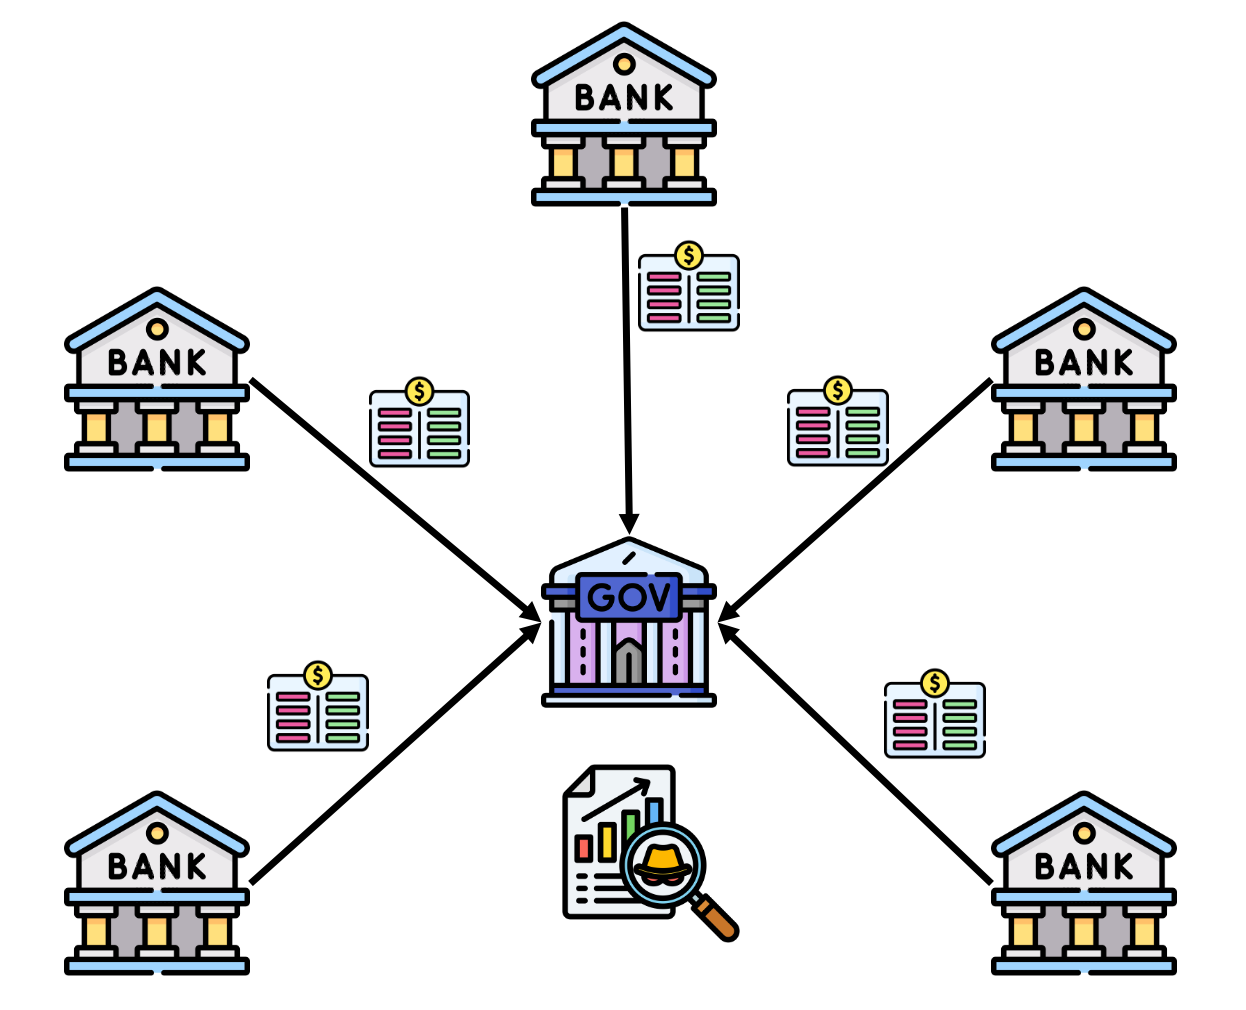
\includegraphics[width=0.4\textwidth]{img/crs.png}
    \end{center}
\end{frame}


\begin{frame}
    \frametitle{Implementación de un caso de uso}

    
    \begin{block}{Descripción}
       
        Una jerarquía de directorios en un sistema operativo es una estructura de organización y almacenamiento de archivos y carpetas (directorios) en forma de árbol. Esta estructura permite a los usuarios y programas almacenar y acceder a los archivos de manera ordenada.

    \end{block}
    % \note<2>{@NOTE x ejemplo:
    %     \begin{itemize}
    %         \item referenciar a valores \'unicos
    %         \item eliminar redundancia en datos repetidos continuamente (Run-Length Encoding)
    %         \item eliminaci\'on de nulls llevando m\'ascaras de bits, por ejemplo
    %     \end{itemize}
    % }

    \begin{center}
        
        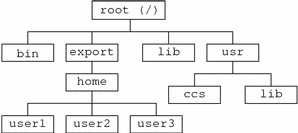
\includegraphics[width=0.4\textwidth]{img/directories.png}
    \end{center}
\end{frame}


% \begin{frame}
%     \frametitle{Implementación de un caso de uso}

%     \begin{block}{Requerimientos}
%         \begin{itemize}
%             \item \textbf{Simplicidad conceptual}: Solo es necesario almacenar los nombres de dominio y las direcciones IP. Además las consultas se limitan a obtener el IP asociado a un nombre de dominio.
%             \item \textbf{Gran volumen de operaciones}: El escenario es muy dinámico, con dispositivos entrando y saliendo de la red mientras se comunican entre sí (es decir, deben de buscar sus IPs).
%             \item \textbf{Alta disponibilidad}: La caída de un sistema DNS significaría la interrupción de una gran parte de las comunicaciones en la red, por tanto se debe garantizar la disponibilidad del sistema.
%         \end{itemize}

%     \end{block}

% \end{frame}


\begin{frame}
    \frametitle{Implementación de un caso de uso}

    \begin{block}{Código}
        El código para simular y solucionar el escenario se encuentra en uno de los repositorios
        de la disciplina \href{https://github.com/ISBIG-UH/no-sql-samples/}{https://github.com/ISBIG-UH/no-sql-samples/}

        \begin{center}
            
            
\includegraphics[width=40mm]{img/repo-qrcode.png}
        \end{center}
   
    \end{block}

\end{frame}



